\documentclass[tikz]{standalone}
\usepackage{tikz}
\usepackage{graphics}
\usepackage{color}
\usepackage{tikz}
\usetikzlibrary{patterns}
\usetikzlibrary{shapes}
\usetikzlibrary{arrows.meta,arrows}


%%%%%%%%%%%%%%%%%%%%%%%%%%%%%%%%%%%%%%%%%%%%%%%%%%%%%%%%%%%%%%%%%%%%%%%%%%%%%%%%%%%%

%%%  latex --shell-escape CasLevcek.tex

%%%%%%%%%%%%%%%%%%%%%%%%%%%%%%%%%%%%%%%%%%%%%%%%%%%%%%%%%%%%%%%%%%%%%%%%%%%%%%%%%%%%

\usepackage{amssymb} 		%%pour faire lessim
\usepackage{amsmath}		%%pour faire equation*
\usepackage{amsthm} 		%%environnement théorème (!!!)
\usepackage{array,multirow,makecell}

% \usetikzlibrary{external} % set up externalization

% \tikzexternalize[shell escape=-enable-write18] % activate externalisation

% \tikzset{external/system call={latex \tikzexternalcheckshellescape -halt-on-error
		% -interaction=batchmode -jobname "\image" "\texsource" && 
		% dvips -o "\image".ps "\image".dvi &&
		% ps2eps -l "\image.ps"}}


\newcommand{\aaA}{1.5}
\newcommand{\aaB}{3}
\newcommand{\aaC}{4.5}
\newcommand{\aaD}{6}

\begin{document}
		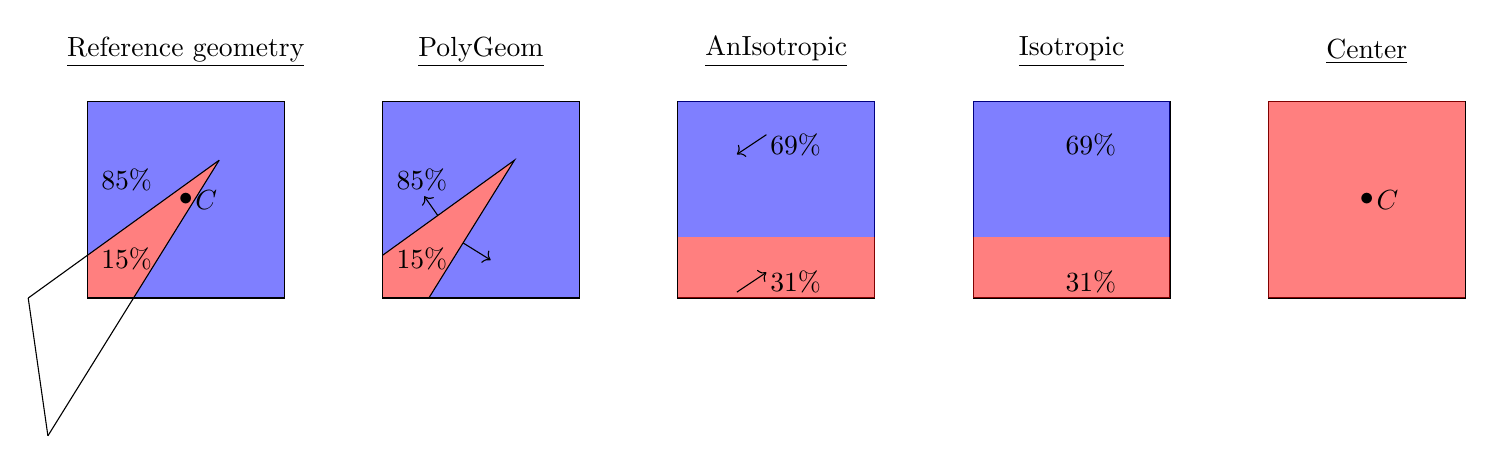
\begin{tikzpicture}[scale = 2.5]

		\fill [color = red, opacity=0.5](0, 0.217)--(0.67, 0.7)--(0.235, 0)--(0,0)--cycle;
		\fill [color = blue, opacity=0.5] (1, 0) -- (1,1) -- (0,1)--(0, 0.217)--(0.67, 0.7)--(0.235, 0)--cycle;
		
		\draw (0, 0) rectangle (1, 1);
		\draw (0.5, 0.5) node {$\bullet$};
		\draw (0.5, 0.5) node[right] {$C$};
		
		\draw (-0.3, 0)--(0.67, 0.7);
		\draw (-0.2, -0.7)--(0.67, 0.7);
		\draw (-0.2, -0.7)--(-0.3, 0);
		
		\draw (0.2, 0.2)node {$15\%$};
		\draw (0.2, 0.6)node {$85\%$};		
		% Poly Geom
		\fill [color = red, opacity=0.5](\aaA+0, 0.217)--(\aaA+0.67, 0.7)--(\aaA+0.235, 0)--(\aaA+0,0)--cycle;
		\fill [color = blue, opacity=0.5] (\aaA+1, 0) -- (\aaA+1,1) -- (\aaA+0,1)--(\aaA+0, 0.217)--(\aaA+0.67, 0.7)--(\aaA+0.235, 0)--cycle;
		\draw (\aaA+0, 0) rectangle (\aaA+1, 1);		
		\draw (\aaA+0, 0.217)--(\aaA+0.67, 0.7)--(\aaA+0.235, 0);
		\draw (\aaA+0.2, 0.2)node {$15\%$};
		\draw (\aaA+0.2, 0.6)node {$85\%$};
		\draw[->] (\aaA+0.28, 0.42)--(\aaA+0.212, 0.517);
		\draw[->] (\aaA+0.409, 0.28)--(\aaA+0.549, 0.193);		
		% AnIso
		\draw (\aaB+0, 0) rectangle (\aaB+1, 1);		
		\draw (\aaB+0, 0) rectangle (\aaB+1, 1);		
		\fill [color = blue, opacity=0.5] (\aaB+0, 1)--(\aaB+0,0.31) -- (\aaB+1,0.31) -- (\aaB+1,1)--cycle;
		\fill [color = red, opacity=0.5] (\aaB+0, 0)--(\aaB+0,0.31) -- (\aaB+1,0.31) -- (\aaB+1,0)--cycle;		
		\draw[->] (\aaB+0.45, 0.83)--(\aaB+0.3, 0.73);
		\draw (\aaB+0.42, 0.78) node[right] {$69\%$};		
		\draw[->] (\aaB+0.3, 0.03)--(\aaB+0.45, 0.13);
		\draw (\aaB+0.42, 0.08) node[right] {$31\%$};
		% Iso
		\draw (\aaC+0, 0) rectangle (\aaC+1, 1);		
		\draw (\aaC+0, 0) rectangle (\aaC+1, 1);		
		\fill [color = blue, opacity=0.5] (\aaC+0, 1)--(\aaC+0,0.31) -- (\aaC+1,0.31) -- (\aaC+1,1)--cycle;
		\fill [color = red, opacity=0.5] (\aaC+0, 0)--(\aaC+0,0.31) -- (\aaC+1,0.31) -- (\aaC+1,0)--cycle;		
		\draw (\aaC+0.42, 0.78) node[right] {$69\%$};
		\draw (\aaC+0.42, 0.08) node[right] {$31\%$};		
		% Center
		\draw (\aaD+0, 0) rectangle (\aaD+1, 1);
		\draw (\aaD+0, 0) rectangle (\aaD+1, 1);
		\fill [color = red, opacity=0.5] (\aaD+0, 0) rectangle (\aaD+1, 1);		
		\draw (\aaD+0.5, 0.5) node {$\bullet$};
		\draw (\aaD+0.5, 0.5) node[right] {$C$};
		%
		\draw (0.5, 1.25) node {\underline{Reference geometry}};
		\draw (0.5 + \aaA, 1.25) node {\underline{PolyGeom}};
		\draw (0.5 + \aaB, 1.25) node {\underline{AnIsotropic}};
		\draw (0.5 + \aaC, 1.25) node {\underline{Isotropic}};
		\draw (0.5 + \aaD, 1.25) node {\underline{Center}};
	\end{tikzpicture}
\end{document}
